% Options for packages loaded elsewhere
% Options for packages loaded elsewhere
\PassOptionsToPackage{unicode}{hyperref}
\PassOptionsToPackage{hyphens}{url}
\PassOptionsToPackage{dvipsnames,svgnames,x11names}{xcolor}
%
\documentclass[
  letterpaper,
  DIV=11,
  numbers=noendperiod]{scrreprt}
\usepackage{xcolor}
\usepackage{amsmath,amssymb}
\setcounter{secnumdepth}{5}
\usepackage{iftex}
\ifPDFTeX
  \usepackage[T1]{fontenc}
  \usepackage[utf8]{inputenc}
  \usepackage{textcomp} % provide euro and other symbols
\else % if luatex or xetex
  \usepackage{unicode-math} % this also loads fontspec
  \defaultfontfeatures{Scale=MatchLowercase}
  \defaultfontfeatures[\rmfamily]{Ligatures=TeX,Scale=1}
\fi
\usepackage{lmodern}
\ifPDFTeX\else
  % xetex/luatex font selection
\fi
% Use upquote if available, for straight quotes in verbatim environments
\IfFileExists{upquote.sty}{\usepackage{upquote}}{}
\IfFileExists{microtype.sty}{% use microtype if available
  \usepackage[]{microtype}
  \UseMicrotypeSet[protrusion]{basicmath} % disable protrusion for tt fonts
}{}
\makeatletter
\@ifundefined{KOMAClassName}{% if non-KOMA class
  \IfFileExists{parskip.sty}{%
    \usepackage{parskip}
  }{% else
    \setlength{\parindent}{0pt}
    \setlength{\parskip}{6pt plus 2pt minus 1pt}}
}{% if KOMA class
  \KOMAoptions{parskip=half}}
\makeatother
% Make \paragraph and \subparagraph free-standing
\makeatletter
\ifx\paragraph\undefined\else
  \let\oldparagraph\paragraph
  \renewcommand{\paragraph}{
    \@ifstar
      \xxxParagraphStar
      \xxxParagraphNoStar
  }
  \newcommand{\xxxParagraphStar}[1]{\oldparagraph*{#1}\mbox{}}
  \newcommand{\xxxParagraphNoStar}[1]{\oldparagraph{#1}\mbox{}}
\fi
\ifx\subparagraph\undefined\else
  \let\oldsubparagraph\subparagraph
  \renewcommand{\subparagraph}{
    \@ifstar
      \xxxSubParagraphStar
      \xxxSubParagraphNoStar
  }
  \newcommand{\xxxSubParagraphStar}[1]{\oldsubparagraph*{#1}\mbox{}}
  \newcommand{\xxxSubParagraphNoStar}[1]{\oldsubparagraph{#1}\mbox{}}
\fi
\makeatother

\usepackage{color}
\usepackage{fancyvrb}
\newcommand{\VerbBar}{|}
\newcommand{\VERB}{\Verb[commandchars=\\\{\}]}
\DefineVerbatimEnvironment{Highlighting}{Verbatim}{commandchars=\\\{\}}
% Add ',fontsize=\small' for more characters per line
\usepackage{framed}
\definecolor{shadecolor}{RGB}{241,243,245}
\newenvironment{Shaded}{\begin{snugshade}}{\end{snugshade}}
\newcommand{\AlertTok}[1]{\textcolor[rgb]{0.68,0.00,0.00}{#1}}
\newcommand{\AnnotationTok}[1]{\textcolor[rgb]{0.37,0.37,0.37}{#1}}
\newcommand{\AttributeTok}[1]{\textcolor[rgb]{0.40,0.45,0.13}{#1}}
\newcommand{\BaseNTok}[1]{\textcolor[rgb]{0.68,0.00,0.00}{#1}}
\newcommand{\BuiltInTok}[1]{\textcolor[rgb]{0.00,0.23,0.31}{#1}}
\newcommand{\CharTok}[1]{\textcolor[rgb]{0.13,0.47,0.30}{#1}}
\newcommand{\CommentTok}[1]{\textcolor[rgb]{0.37,0.37,0.37}{#1}}
\newcommand{\CommentVarTok}[1]{\textcolor[rgb]{0.37,0.37,0.37}{\textit{#1}}}
\newcommand{\ConstantTok}[1]{\textcolor[rgb]{0.56,0.35,0.01}{#1}}
\newcommand{\ControlFlowTok}[1]{\textcolor[rgb]{0.00,0.23,0.31}{\textbf{#1}}}
\newcommand{\DataTypeTok}[1]{\textcolor[rgb]{0.68,0.00,0.00}{#1}}
\newcommand{\DecValTok}[1]{\textcolor[rgb]{0.68,0.00,0.00}{#1}}
\newcommand{\DocumentationTok}[1]{\textcolor[rgb]{0.37,0.37,0.37}{\textit{#1}}}
\newcommand{\ErrorTok}[1]{\textcolor[rgb]{0.68,0.00,0.00}{#1}}
\newcommand{\ExtensionTok}[1]{\textcolor[rgb]{0.00,0.23,0.31}{#1}}
\newcommand{\FloatTok}[1]{\textcolor[rgb]{0.68,0.00,0.00}{#1}}
\newcommand{\FunctionTok}[1]{\textcolor[rgb]{0.28,0.35,0.67}{#1}}
\newcommand{\ImportTok}[1]{\textcolor[rgb]{0.00,0.46,0.62}{#1}}
\newcommand{\InformationTok}[1]{\textcolor[rgb]{0.37,0.37,0.37}{#1}}
\newcommand{\KeywordTok}[1]{\textcolor[rgb]{0.00,0.23,0.31}{\textbf{#1}}}
\newcommand{\NormalTok}[1]{\textcolor[rgb]{0.00,0.23,0.31}{#1}}
\newcommand{\OperatorTok}[1]{\textcolor[rgb]{0.37,0.37,0.37}{#1}}
\newcommand{\OtherTok}[1]{\textcolor[rgb]{0.00,0.23,0.31}{#1}}
\newcommand{\PreprocessorTok}[1]{\textcolor[rgb]{0.68,0.00,0.00}{#1}}
\newcommand{\RegionMarkerTok}[1]{\textcolor[rgb]{0.00,0.23,0.31}{#1}}
\newcommand{\SpecialCharTok}[1]{\textcolor[rgb]{0.37,0.37,0.37}{#1}}
\newcommand{\SpecialStringTok}[1]{\textcolor[rgb]{0.13,0.47,0.30}{#1}}
\newcommand{\StringTok}[1]{\textcolor[rgb]{0.13,0.47,0.30}{#1}}
\newcommand{\VariableTok}[1]{\textcolor[rgb]{0.07,0.07,0.07}{#1}}
\newcommand{\VerbatimStringTok}[1]{\textcolor[rgb]{0.13,0.47,0.30}{#1}}
\newcommand{\WarningTok}[1]{\textcolor[rgb]{0.37,0.37,0.37}{\textit{#1}}}

\usepackage{longtable,booktabs,array}
\newcounter{none} % for unnumbered tables
\usepackage{calc} % for calculating minipage widths
% Correct order of tables after \paragraph or \subparagraph
\usepackage{etoolbox}
\makeatletter
\patchcmd\longtable{\par}{\if@noskipsec\mbox{}\fi\par}{}{}
\makeatother
% Allow footnotes in longtable head/foot
\IfFileExists{footnotehyper.sty}{\usepackage{footnotehyper}}{\usepackage{footnote}}
\makesavenoteenv{longtable}
\usepackage{graphicx}
\makeatletter
\newsavebox\pandoc@box
\newcommand*\pandocbounded[1]{% scales image to fit in text height/width
  \sbox\pandoc@box{#1}%
  \Gscale@div\@tempa{\textheight}{\dimexpr\ht\pandoc@box+\dp\pandoc@box\relax}%
  \Gscale@div\@tempb{\linewidth}{\wd\pandoc@box}%
  \ifdim\@tempb\p@<\@tempa\p@\let\@tempa\@tempb\fi% select the smaller of both
  \ifdim\@tempa\p@<\p@\scalebox{\@tempa}{\usebox\pandoc@box}%
  \else\usebox{\pandoc@box}%
  \fi%
}
% Set default figure placement to htbp
\def\fps@figure{htbp}
\makeatother





\setlength{\emergencystretch}{3em} % prevent overfull lines

\providecommand{\tightlist}{%
  \setlength{\itemsep}{0pt}\setlength{\parskip}{0pt}}



 


\KOMAoption{captions}{tableheading}
\makeatletter
\@ifpackageloaded{bookmark}{}{\usepackage{bookmark}}
\makeatother
\makeatletter
\@ifpackageloaded{caption}{}{\usepackage{caption}}
\AtBeginDocument{%
\ifdefined\contentsname
  \renewcommand*\contentsname{Table of contents}
\else
  \newcommand\contentsname{Table of contents}
\fi
\ifdefined\listfigurename
  \renewcommand*\listfigurename{List of Figures}
\else
  \newcommand\listfigurename{List of Figures}
\fi
\ifdefined\listtablename
  \renewcommand*\listtablename{List of Tables}
\else
  \newcommand\listtablename{List of Tables}
\fi
\ifdefined\figurename
  \renewcommand*\figurename{Figure}
\else
  \newcommand\figurename{Figure}
\fi
\ifdefined\tablename
  \renewcommand*\tablename{Table}
\else
  \newcommand\tablename{Table}
\fi
}
\@ifpackageloaded{float}{}{\usepackage{float}}
\floatstyle{ruled}
\@ifundefined{c@chapter}{\newfloat{codelisting}{h}{lop}}{\newfloat{codelisting}{h}{lop}[chapter]}
\floatname{codelisting}{Listing}
\newcommand*\listoflistings{\listof{codelisting}{List of Listings}}
\makeatother
\makeatletter
\makeatother
\makeatletter
\@ifpackageloaded{caption}{}{\usepackage{caption}}
\@ifpackageloaded{subcaption}{}{\usepackage{subcaption}}
\makeatother
\usepackage{bookmark}
\IfFileExists{xurl.sty}{\usepackage{xurl}}{} % add URL line breaks if available
\urlstyle{same}
% fallback for those not using the hyperref driver hyperxmp:
\makeatletter
\@ifundefined{xmpquote}{\newcommand{\xmpquote}[1]{#1}}{}
\makeatother
\hypersetup{
  pdftitle={Bioarchaeology Visualization},
  pdfauthor={Jen Heilmann},
  colorlinks=true,
  linkcolor={blue},
  filecolor={Maroon},
  citecolor={Blue},
  urlcolor={Blue},
  pdfcreator={LaTeX via pandoc}}


\title{Bioarchaeology Visualization}
\author{Jen Heilmann}
\date{2026-09-26}
\begin{document}
\maketitle

\renewcommand*\contentsname{Table of contents}
{
\setcounter{tocdepth}{2}
\tableofcontents
}

\bookmarksetup{startatroot}

\chapter*{Overview}\label{overview}
\addcontentsline{toc}{chapter}{Overview}

\markboth{Overview}{Overview}

\section*{Purpose}\label{purpose}
\addcontentsline{toc}{section}{Purpose}

\markright{Purpose}

This book is an open-access resource for students and professionals who
want to create clear, accurate, and publication-ready visualizations of
bioarchaeological data using R and ggplot2

\section*{Sections}\label{sections}
\addcontentsline{toc}{section}{Sections}

\markright{Sections}

The book is divided into two main parts:

\begin{enumerate}
\def\labelenumi{\arabic{enumi}.}
\tightlist
\item
  Introduction to R Visualizations
\item
  Discipline-Specific Visualizations
\end{enumerate}

\section*{Goals}\label{goals}
\addcontentsline{toc}{section}{Goals}

\markright{Goals}

\begin{enumerate}
\def\labelenumi{\arabic{enumi}.}
\tightlist
\item
  \textbf{Locate and access} open databases and R packages relevant to
  isotopic analysis, geometric morphometrics, and spatial data in
  bioarchaeology.
\item
  \textbf{Select} appropriate visualization types based on the data
  structure and the research question being asked.
\item
  \textbf{Interpret} each type of visualization, recognizing what the
  plot shows, what it does not show, and common pitfalls in reading it.
\item
  \textbf{Adapt} the annotated code examples to individual datasets and
  research projects.
\end{enumerate}

\part{R Basics}

\chapter{Summary Statistics}\label{summary-statistics}

\chapter{Data Frames}\label{data-frames}

\chapter{Custom Functions}\label{custom-functions}

\part{Data Analysis}

\chapter{Hypothesis Testing}\label{hypothesis-testing}

\chapter{ANOVA}\label{anova}

\chapter{Regression}\label{regression}

\part{Introduction to Visualization}

\chapter*{Types of Visualizations}\label{types-of-visualizations}
\addcontentsline{toc}{chapter}{Types of Visualizations}

\markboth{Types of Visualizations}{Types of Visualizations}

\section*{Distribution}\label{distribution}
\addcontentsline{toc}{section}{Distribution}

\markright{Distribution}

\subsection*{Boxplot}\label{boxplot}
\addcontentsline{toc}{subsection}{Boxplot}

\begin{Shaded}
\begin{Highlighting}[]
\FunctionTok{library}\NormalTok{(ggplot2)}
\FunctionTok{ggplot}\NormalTok{(data, }\FunctionTok{aes}\NormalTok{(}\AttributeTok{y=}\NormalTok{value))}\SpecialCharTok{+}
  \FunctionTok{geom\_boxplot}\NormalTok{()}
\end{Highlighting}
\end{Shaded}

\begin{figure}[H]

{\centering \pandocbounded{\includegraphics[keepaspectratio]{Types_files/figure-pdf/basic-boxplot-1.pdf}}

}

\caption{Basic Boxplot}

\end{figure}%

\begin{Shaded}
\begin{Highlighting}[]
\FunctionTok{ggplot}\NormalTok{(data, }\FunctionTok{aes}\NormalTok{(}\AttributeTok{y=}\NormalTok{value, }\AttributeTok{x=}\NormalTok{group))}\SpecialCharTok{+}
  \FunctionTok{geom\_boxplot}\NormalTok{()}
\end{Highlighting}
\end{Shaded}

\begin{figure}[H]

{\centering \pandocbounded{\includegraphics[keepaspectratio]{Types_files/figure-pdf/group-boxplot-1.pdf}}

}

\caption{Boxplot by Group}

\end{figure}%

\subsection*{Violin}\label{violin}
\addcontentsline{toc}{subsection}{Violin}

\begin{Shaded}
\begin{Highlighting}[]
\FunctionTok{ggplot}\NormalTok{(data, }\FunctionTok{aes}\NormalTok{(}\AttributeTok{x=}\NormalTok{group, }\AttributeTok{y=}\NormalTok{value))}\SpecialCharTok{+}
  \FunctionTok{geom\_violin}\NormalTok{()}
\end{Highlighting}
\end{Shaded}

\begin{figure}[H]

{\centering \pandocbounded{\includegraphics[keepaspectratio]{Types_files/figure-pdf/violin-1.pdf}}

}

\caption{Violin Plot by Group}

\end{figure}%

\subsection*{Histogram}\label{histogram}
\addcontentsline{toc}{subsection}{Histogram}

\begin{Shaded}
\begin{Highlighting}[]
\FunctionTok{ggplot}\NormalTok{(data, }\FunctionTok{aes}\NormalTok{(}\AttributeTok{x=}\NormalTok{value))}\SpecialCharTok{+}
  \FunctionTok{geom\_histogram}\NormalTok{()}
\end{Highlighting}
\end{Shaded}

\begin{figure}[H]

{\centering \pandocbounded{\includegraphics[keepaspectratio]{Types_files/figure-pdf/basic-histogram-1.pdf}}

}

\caption{Basic Histogram}

\end{figure}%

\begin{Shaded}
\begin{Highlighting}[]
\FunctionTok{ggplot}\NormalTok{(data, }\FunctionTok{aes}\NormalTok{(}\AttributeTok{x=}\NormalTok{value))}\SpecialCharTok{+}
  \FunctionTok{geom\_histogram}\NormalTok{(}\AttributeTok{binwidth=}\NormalTok{.}\DecValTok{1}\NormalTok{)}
\end{Highlighting}
\end{Shaded}

\begin{figure}[H]

{\centering \pandocbounded{\includegraphics[keepaspectratio]{Types_files/figure-pdf/bin-histogram-1.pdf}}

}

\caption{Histogram with designated Bins}

\end{figure}%

\subsection*{Density}\label{density}
\addcontentsline{toc}{subsection}{Density}

\begin{Shaded}
\begin{Highlighting}[]
\FunctionTok{ggplot}\NormalTok{(data, }\FunctionTok{aes}\NormalTok{(}\AttributeTok{x=}\NormalTok{value))}\SpecialCharTok{+}
  \FunctionTok{geom\_density}\NormalTok{()}
\end{Highlighting}
\end{Shaded}

\pandocbounded{\includegraphics[keepaspectratio]{Types_files/figure-pdf/density-1.pdf}}

\section*{Correlation}\label{correlation}
\addcontentsline{toc}{section}{Correlation}

\markright{Correlation}

\subsection*{Scatter}\label{scatter}
\addcontentsline{toc}{subsection}{Scatter}

\subsection*{Bubble}\label{bubble}
\addcontentsline{toc}{subsection}{Bubble}

\subsection*{Heatmap}\label{heatmap}
\addcontentsline{toc}{subsection}{Heatmap}

\subsection*{Correlogram}\label{correlogram}
\addcontentsline{toc}{subsection}{Correlogram}

\section*{Map}\label{map}
\addcontentsline{toc}{section}{Map}

\markright{Map}

\subsection*{Map}\label{map-1}
\addcontentsline{toc}{subsection}{Map}

\subsection*{Choropleth}\label{choropleth}
\addcontentsline{toc}{subsection}{Choropleth}

\subsection*{Bubble Map}\label{bubble-map}
\addcontentsline{toc}{subsection}{Bubble Map}

\section*{Flow}\label{flow}
\addcontentsline{toc}{section}{Flow}

\markright{Flow}

\subsection*{Chord Diagram}\label{chord-diagram}
\addcontentsline{toc}{subsection}{Chord Diagram}

\subsection*{Network}\label{network}
\addcontentsline{toc}{subsection}{Network}

\subsection*{Sankey}\label{sankey}
\addcontentsline{toc}{subsection}{Sankey}

\subsection*{Dendrogram}\label{dendrogram}
\addcontentsline{toc}{subsection}{Dendrogram}

\chapter{Visualization Packages}\label{visualization-packages}

\chapter{Customizing Plots}\label{customizing-plots}

\part{Stable Isotope Analysis}

\chapter*{Resources}\label{resources}
\addcontentsline{toc}{chapter}{Resources}

\markboth{Resources}{Resources}

\section*{Isotope Databases}\label{isotope-databases}
\addcontentsline{toc}{section}{Isotope Databases}

\markright{Isotope Databases}

\href{https://pandoradata.earth/my_MM/dataset/maia}{MAIA}: Mediterranean
Archive of Isotopic Data

\href{https://pandora.earth/mn_MN/dataset/isotopia-a-stable-isotope-database-for-classical-antiquity}{Isotòpia}:
A stable isotope database for Classical Antiquity

\href{https://www.seanoe.org/data/00895/100661/}{ISOMED}: A stable
isotope database of Mediterranean marine food web components

\href{https://explorer.isoarch.org/}{IsoArcH}: A stable isotope database
for research worldwide

\section*{R Packages for Stable
Isotopes}\label{r-packages-for-stable-isotopes}
\addcontentsline{toc}{section}{R Packages for Stable Isotopes}

\markright{R Packages for Stable Isotopes}

\subsection*{Diet Mixing Models}\label{diet-mixing-models}
\addcontentsline{toc}{subsection}{Diet Mixing Models}

\subsubsection*{simmr: A Stable Isotope Mixing
Model}\label{simmr-a-stable-isotope-mixing-model}
\addcontentsline{toc}{subsubsection}{simmr: A Stable Isotope Mixing
Model}

\href{https://CRAN.R-project.org/package=simmr}{R Project Page}
\textbar{} \href{https://github.com/andrewcparnell/simmr}{GitHub Page}

\subsubsection*{cosimmr: Fast Fitting of Stable Isotope Mixing Models
with
Covariates}\label{cosimmr-fast-fitting-of-stable-isotope-mixing-models-with-covariates}
\addcontentsline{toc}{subsubsection}{cosimmr: Fast Fitting of Stable
Isotope Mixing Models with Covariates}

\href{https://CRAN.R-project.org/package=cosimmr}{R Project Page}
\textbar{} \href{https://github.com/emmagovan/cosimmr}{GitHub Page}

\subsubsection*{MixSIAR: Bayesian Mixing Models in
R}\label{mixsiar-bayesian-mixing-models-in-r}
\addcontentsline{toc}{subsubsection}{MixSIAR: Bayesian Mixing Models in
R}

\href{https://CRAN.R-project.org/package=MixSIAR}{R Project Page}
\textbar{} \href{https://github.com/brianstock/MixSIAR}{GitHub Page}

\subsubsection*{ReSources: Food Reconstruction Using Isotopic
Transferred
Signals}\label{resources-food-reconstruction-using-isotopic-transferred-signals}
\addcontentsline{toc}{subsubsection}{ReSources: Food Reconstruction
Using Isotopic Transferred Signals}

\href{https://pandora-isomemo.github.io/docs/apps.html}{IsoMemo Page}
\textbar{} \href{https://github.com/Pandora-IsoMemo/ReSources}{GitHub
Page}

\subsection*{Isoscapes}\label{isoscapes}
\addcontentsline{toc}{subsection}{Isoscapes}

\subsubsection*{assignR: Infer Geographic Origin from Isotopic
Data}\label{assignr-infer-geographic-origin-from-isotopic-data}
\addcontentsline{toc}{subsubsection}{assignR: Infer Geographic Origin
from Isotopic Data}

\href{https://CRAN.R-project.org/package=assignR}{R Project Page}

\subsubsection*{IsoriX: Isoscape Computation and Inference of Spatial
Origins using Mixed
Models}\label{isorix-isoscape-computation-and-inference-of-spatial-origins-using-mixed-models}
\addcontentsline{toc}{subsubsection}{IsoriX: Isoscape Computation and
Inference of Spatial Origins using Mixed Models}

\href{https://CRAN.R-project.org/package=IsoriX}{R Project Page}
\textbar{} \href{https://github.com/courtiol/IsoriX}{GitHub Page}

\subsubsection*{isocat: Isotope Origin Clustering and Assignment
Tools}\label{isocat-isotope-origin-clustering-and-assignment-tools}
\addcontentsline{toc}{subsubsection}{isocat: Isotope Origin Clustering
and Assignment Tools}

\href{https://CRAN.R-project.org/package=isocat}{R Project Page}
\textbar{} \href{https://github.com/cjcampbell/isocat}{GitHub Page}

\chapter{Trace Element Analysis}\label{trace-element-analysis}

\section{Checking for Diagenesis}\label{checking-for-diagenesis}

\subsection{Maximum Threshold Concentration
(MTC)}\label{maximum-threshold-concentration-mtc}

Source: Kamenov et al., 2018

\begin{Shaded}
\begin{Highlighting}[]
\FunctionTok{library}\NormalTok{(gt)}
\FunctionTok{library}\NormalTok{(dplyr)}

\NormalTok{Elements }\OtherTok{\textless{}{-}} \FunctionTok{c}\NormalTok{(}\StringTok{"Mg"}\NormalTok{, }\StringTok{"Ca"}\NormalTok{, }\StringTok{"V"}\NormalTok{, }\StringTok{"Cr"}\NormalTok{, }\StringTok{"Mn"}\NormalTok{, }\StringTok{"Fe"}\NormalTok{, }\StringTok{"Ni"}\NormalTok{, }\StringTok{"Cu"}\NormalTok{, }\StringTok{"Zn"}\NormalTok{, }\StringTok{"Sr"}\NormalTok{,}
              \StringTok{"Ba"}\NormalTok{, }\StringTok{"La"}\NormalTok{, }\StringTok{"Ce"}\NormalTok{, }\StringTok{"Pr"}\NormalTok{, }\StringTok{"Nd"}\NormalTok{, }\StringTok{"Sm"}\NormalTok{, }\StringTok{"Eu"}\NormalTok{,}\StringTok{"Gd"}\NormalTok{ , }\StringTok{"Tb"}\NormalTok{, }\StringTok{"Dy"}\NormalTok{,}
              \StringTok{"Ho"}\NormalTok{, }\StringTok{"Er"}\NormalTok{, }\StringTok{"Tm"}\NormalTok{, }\StringTok{"Yb"}\NormalTok{, }\StringTok{"Lu"}\NormalTok{, }\StringTok{"Pb"}\NormalTok{, }\StringTok{"Th"}\NormalTok{, }\StringTok{"U"}\NormalTok{)}

\NormalTok{MTC }\OtherTok{\textless{}{-}} \FunctionTok{c}\NormalTok{(}\DecValTok{6472}\NormalTok{, }\DecValTok{462387}\NormalTok{, }\FloatTok{0.11}\NormalTok{, }\FloatTok{13.9}\NormalTok{, }\FloatTok{15.4}\NormalTok{, }\DecValTok{143}\NormalTok{, }\DecValTok{46}\NormalTok{, }\DecValTok{48}\NormalTok{, }\DecValTok{629}\NormalTok{, }\DecValTok{1700}\NormalTok{,}
         \DecValTok{40}\NormalTok{, }\FloatTok{0.1}\NormalTok{, }\FloatTok{0.12}\NormalTok{, }\FloatTok{0.015}\NormalTok{, }\FloatTok{0.058}\NormalTok{, }\FloatTok{0.030}\NormalTok{, }\ConstantTok{NA}\NormalTok{, }\ConstantTok{NA}\NormalTok{, }\FloatTok{0.002}\NormalTok{, }\FloatTok{0.009}\NormalTok{,}
         \FloatTok{0.002}\NormalTok{, }\FloatTok{0.008}\NormalTok{, }\FloatTok{0.001}\NormalTok{, }\FloatTok{0.021}\NormalTok{, }\FloatTok{0.003}\NormalTok{, }\DecValTok{63}\NormalTok{, }\FloatTok{0.05}\NormalTok{, }\FloatTok{0.05}\NormalTok{)}

\NormalTok{trace }\OtherTok{\textless{}{-}} \FunctionTok{data.frame}\NormalTok{(Elements, MTC)}
\end{Highlighting}
\end{Shaded}

\subsection{Normalizing your data (divide by the
MTC)}\label{normalizing-your-data-divide-by-the-mtc}

\begin{enumerate}
\def\labelenumi{\arabic{enumi}.}
\tightlist
\item
  Transform data into a wide format
\end{enumerate}

\begin{Shaded}
\begin{Highlighting}[]
\CommentTok{\# Depending on the format of your data, transform the dataframe so that the rows represent the samples/individuals and the columns represent the trace elements.}
\end{Highlighting}
\end{Shaded}

\begin{enumerate}
\def\labelenumi{\arabic{enumi}.}
\setcounter{enumi}{1}
\tightlist
\item
  Normalize each column by dividing by the MTC
\end{enumerate}

\begin{Shaded}
\begin{Highlighting}[]
\NormalTok{mtc }\OtherTok{\textless{}{-}}\NormalTok{ trace}\SpecialCharTok{$}\NormalTok{MTC[}\FunctionTok{match}\NormalTok{(}\FunctionTok{names}\NormalTok{(enamel)[}\SpecialCharTok{{-}}\DecValTok{1}\NormalTok{], trace}\SpecialCharTok{$}\NormalTok{Elements)] }\CommentTok{\# ensures the elements are in the same order}
\NormalTok{mtc }\OtherTok{\textless{}{-}}\NormalTok{ trace}\SpecialCharTok{$}\NormalTok{MTC[}\FunctionTok{match}\NormalTok{(}\FunctionTok{names}\NormalTok{(enamel)[}\SpecialCharTok{{-}}\DecValTok{1}\NormalTok{], trace}\SpecialCharTok{$}\NormalTok{Elements)] }
\CommentTok{\# ensures the elements are in the same order}
\CommentTok{\# if you have additional variables, exclude those as well in place of [{-}1] which removes the first column of sample names}

\NormalTok{mtc.ratio }\OtherTok{\textless{}{-}} \FunctionTok{cbind}\NormalTok{(}\AttributeTok{sample=}\NormalTok{enamel}\SpecialCharTok{$}\NormalTok{sample, }\FunctionTok{sweep}\NormalTok{(enamel[,}\SpecialCharTok{{-}}\DecValTok{1}\NormalTok{], }\DecValTok{2}\NormalTok{, mtc, }\StringTok{"/"}\NormalTok{)) }
\CommentTok{\# divides the sample values by the matched MTC values}
\CommentTok{\# sweep(x, Margin, Stats, Fun)}
\end{Highlighting}
\end{Shaded}

\begin{enumerate}
\def\labelenumi{\arabic{enumi}.}
\setcounter{enumi}{2}
\tightlist
\item
  Create a subset of Ratios
\end{enumerate}

\begin{Shaded}
\begin{Highlighting}[]
\FunctionTok{library}\NormalTok{(tidyr)}

\NormalTok{elements }\OtherTok{\textless{}{-}} \FunctionTok{c}\NormalTok{(}\StringTok{"V"}\NormalTok{, }\StringTok{"Mn"}\NormalTok{, }\StringTok{"Fe"}\NormalTok{, }\StringTok{"La"}\NormalTok{, }\StringTok{"Ce"}\NormalTok{, }\StringTok{"Nd"}\NormalTok{, }\StringTok{"Dy"}\NormalTok{, }\StringTok{"Yb"}\NormalTok{, }\StringTok{"Th"}\NormalTok{, }\StringTok{"U"}\NormalTok{)}

\NormalTok{mtc.long }\OtherTok{\textless{}{-}}\NormalTok{ mtc.ratio }\SpecialCharTok{\%\textgreater{}\%}
  \FunctionTok{select}\NormalTok{(sample, }\FunctionTok{all\_of}\NormalTok{(elements)) }\SpecialCharTok{\%\textgreater{}\%} 
  \CommentTok{\# pulls the sample numbers and the values for the subset of elements}
  \FunctionTok{pivot\_longer}\NormalTok{(}\SpecialCharTok{{-}}\NormalTok{sample, }\AttributeTok{names\_to =} \StringTok{"element"}\NormalTok{, }\AttributeTok{values\_to =} \StringTok{"ratio"}\NormalTok{) }
  \CommentTok{\# transforms the table into a stacked format}
\end{Highlighting}
\end{Shaded}

\begin{enumerate}
\def\labelenumi{\arabic{enumi}.}
\setcounter{enumi}{3}
\tightlist
\item
  Plotting the Normalized Concentrations
\end{enumerate}

\begin{Shaded}
\begin{Highlighting}[]
\FunctionTok{library}\NormalTok{(ggplot2)}

\FunctionTok{ggplot}\NormalTok{(mtc.long, }\FunctionTok{aes}\NormalTok{(}\AttributeTok{x=}\NormalTok{sample, }\AttributeTok{y=}\NormalTok{ratio, }\AttributeTok{group=}\NormalTok{element))}\SpecialCharTok{+}
  \FunctionTok{geom\_point}\NormalTok{(}\FunctionTok{aes}\NormalTok{(}\AttributeTok{color=}\NormalTok{element))}\SpecialCharTok{+}
  \FunctionTok{geom\_line}\NormalTok{(}\FunctionTok{aes}\NormalTok{(}\AttributeTok{color=}\NormalTok{element))}\SpecialCharTok{+}
  \FunctionTok{scale\_y\_log10}\NormalTok{() }\SpecialCharTok{+}
  \FunctionTok{geom\_hline}\NormalTok{(}\AttributeTok{yintercept =} \DecValTok{10}\SpecialCharTok{\^{}}\DecValTok{0}\NormalTok{, }\AttributeTok{color=}\StringTok{"red"}\NormalTok{)}\SpecialCharTok{+}
  \FunctionTok{labs}\NormalTok{(}\AttributeTok{x=}\StringTok{"Samples"}\NormalTok{, }\AttributeTok{y=}\StringTok{"C/MTC"}\NormalTok{)}
\end{Highlighting}
\end{Shaded}

\pandocbounded{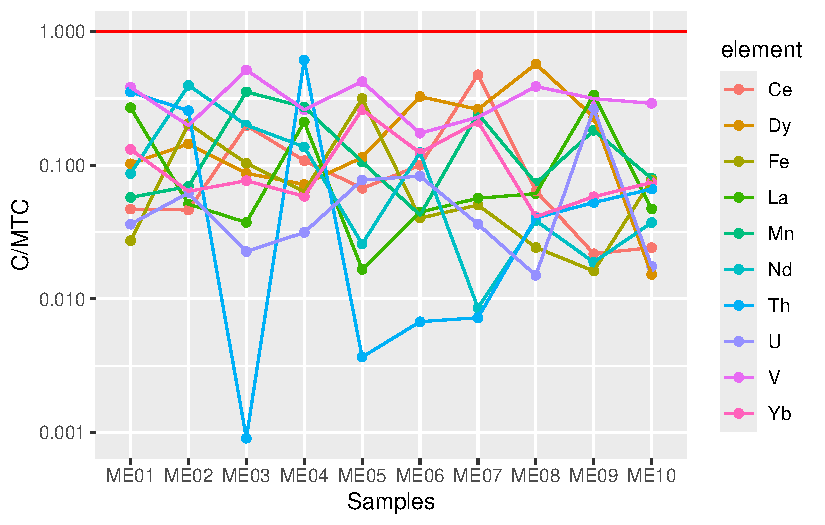
\includegraphics[keepaspectratio]{trace_files/figure-pdf/unnamed-chunk-6-1.pdf}}

\begin{enumerate}
\def\labelenumi{\arabic{enumi}.}
\setcounter{enumi}{4}
\tightlist
\item
  Interpret the Data
\end{enumerate}

\begin{Shaded}
\begin{Highlighting}[]
\CommentTok{\# Dividing the sample concentrations by the maximum threshold concentrations obtained from modern individuals acts as a diagenesis check. If any value exceeds the 10\^{}0 line, there is potential diagenic alteration to the sample.}
\end{Highlighting}
\end{Shaded}

\section{Dietary analysis}\label{dietary-analysis}

Ba/Ca vs.~Sr/Ca

\begin{Shaded}
\begin{Highlighting}[]
\CommentTok{\# Trophic Level and Salinity}
\end{Highlighting}
\end{Shaded}

d13C vs.~Ba/Sr

\begin{Shaded}
\begin{Highlighting}[]
\CommentTok{\# }
\end{Highlighting}
\end{Shaded}

Zn/Ca

\begin{Shaded}
\begin{Highlighting}[]
\CommentTok{\# Proportion of shellfish in diet}
\end{Highlighting}
\end{Shaded}

\chapter{Heavy Isotopes}\label{heavy-isotopes}

\chapter{Light Isotopes}\label{light-isotopes}

\part{Geometric Morphometrics}

\chapter{Generalized Procrustes
Analysis}\label{generalized-procrustes-analysis}

\chapter{Principal Component
Analysis}\label{principal-component-analysis}

\part{Mapping}

\chapter{Basic Maps}\label{basic-maps}

\chapter{Choropleth Maps}\label{choropleth-maps}

\bookmarksetup{startatroot}

\chapter{Summary}\label{summary}

In summary, this book has no content whatsoever.

\begin{Shaded}
\begin{Highlighting}[]
\DecValTok{1} \SpecialCharTok{+} \DecValTok{1}
\end{Highlighting}
\end{Shaded}

\begin{verbatim}
[1] 2
\end{verbatim}

\bookmarksetup{startatroot}

\chapter*{References}\label{references}
\addcontentsline{toc}{chapter}{References}

\markboth{References}{References}

\protect\phantomsection\label{refs}




\end{document}
